%% fig_tangent.tex -- the polarisation turns the tangent space to the Weil
%% family into the annihilator of the Weil line.  Top: the two eigenspaces,
%% each split by Hodge type, and the block matrix of the polarisation between
%% them, which is nonzero on the antidiagonal only.  Middle: the chain of
%% isomorphisms that results.  Right: the three blocks of H^{0,2}.
\documentclass[tikz,border=9pt]{standalone}
\usepackage{amsmath,amssymb}
\usetikzlibrary{arrows.meta,calc,backgrounds,positioning,fit}
%% palette.tex -- shared colour definitions for the figures
\definecolor{PInk}{RGB}{26,32,44}
\definecolor{PBlue}{RGB}{37,82,139}
\definecolor{PTeal}{RGB}{23,127,125}
\definecolor{POchre}{RGB}{193,138,44}
\definecolor{PClay}{RGB}{178,74,58}
\definecolor{PSlate}{RGB}{108,122,137}
\definecolor{PViolet}{RGB}{110,86,150}
\definecolor{WBlue}{RGB}{223,234,246}
\definecolor{WTeal}{RGB}{220,238,236}
\definecolor{WOchre}{RGB}{250,240,218}
\definecolor{WClay}{RGB}{247,229,224}
\definecolor{WSlate}{RGB}{238,241,244}
\definecolor{PMag}{RGB}{158,58,110}
\definecolor{PGrass}{RGB}{62,124,66}
\definecolor{PAmber}{RGB}{214,112,38}
\definecolor{PIndigo}{RGB}{58,64,140}
\definecolor{PRule}{RGB}{176,186,197}

%% shared macros so the standalone figures match the paper
\providecommand{\QQ}{\mathbb{Q}}
\providecommand{\ZZ}{\mathbb{Z}}
\providecommand{\RR}{\mathbb{R}}
\providecommand{\CC}{\mathbb{C}}
\providecommand{\PP}{\mathbb{P}}
\providecommand{\Kx}{K^{\times}}
\providecommand{\HW}{W}
\providecommand{\Nm}{\mathrm{N}}
\providecommand{\Hdg}{\mathrm{Hdg}}
\providecommand{\NS}{\mathrm{NS}}
\providecommand{\cA}{\mathcal{A}}
\providecommand{\cD}{\mathcal{D}}
\providecommand{\cF}{\mathcal{F}}
\providecommand{\cP}{\mathcal{P}}
\providecommand{\cO}{\mathcal{O}}
\providecommand{\cQ}{\mathcal{Q}}
\providecommand{\bbar}[1]{\overline{#1}}
\providecommand{\ch}{\operatorname{ch}}
\providecommand{\End}{\mathrm{End}}


\tikzset{obl/.style={x={(1cm,0cm)}, y={(0.50cm,0.38cm)}, z={(0cm,1cm)}}}

%% a slab: front-bottom-left corner (x0,y0,z0), size (w, dep, h), style prefix
\newcommand{\slab}[7]{%
  \begin{scope}[obl]
    \fill[#7 top]   (#1,#2,#3+#6) -- (#1+#4,#2,#3+#6) -- (#1+#4,#2+#5,#3+#6) -- (#1,#2+#5,#3+#6) -- cycle;
    \fill[#7 front] (#1,#2,#3) -- (#1+#4,#2,#3) -- (#1+#4,#2,#3+#6) -- (#1,#2,#3+#6) -- cycle;
    \fill[#7 side]  (#1+#4,#2,#3) -- (#1+#4,#2+#5,#3) -- (#1+#4,#2+#5,#3+#6) -- (#1+#4,#2,#3+#6) -- cycle;
    \draw[#7 edge]  (#1,#2,#3) -- (#1+#4,#2,#3) -- (#1+#4,#2,#3+#6) -- (#1,#2,#3+#6) -- cycle;
    \draw[#7 edge]  (#1+#4,#2,#3) -- (#1+#4,#2+#5,#3) -- (#1+#4,#2+#5,#3+#6) -- (#1+#4,#2,#3+#6);
    \draw[#7 edge]  (#1,#2,#3+#6) -- (#1,#2+#5,#3+#6) -- (#1+#4,#2+#5,#3+#6);
  \end{scope}}

\tikzset{
  hol top/.style={fill=WBlue},   hol front/.style={fill=WBlue!80!PBlue!30},
  hol side/.style={fill=WBlue!60!PBlue!40},
  hol edge/.style={draw=PBlue,line width=0.6pt},
  ahol top/.style={fill=WClay},  ahol front/.style={fill=WClay!80!PClay!35},
  ahol side/.style={fill=WClay!60!PClay!45},
  ahol edge/.style={draw=PClay,line width=0.6pt},
  mid top/.style={fill=WOchre},  mid front/.style={fill=WOchre!80!POchre!35},
  mid side/.style={fill=WOchre!60!POchre!45},
  mid edge/.style={draw=POchre,line width=0.9pt},
  pale top/.style={fill=WSlate}, pale front/.style={fill=WSlate!80!PSlate!30},
  pale side/.style={fill=WSlate!60!PSlate!40},
  pale edge/.style={draw=PSlate,line width=0.5pt},
}

\begin{document}
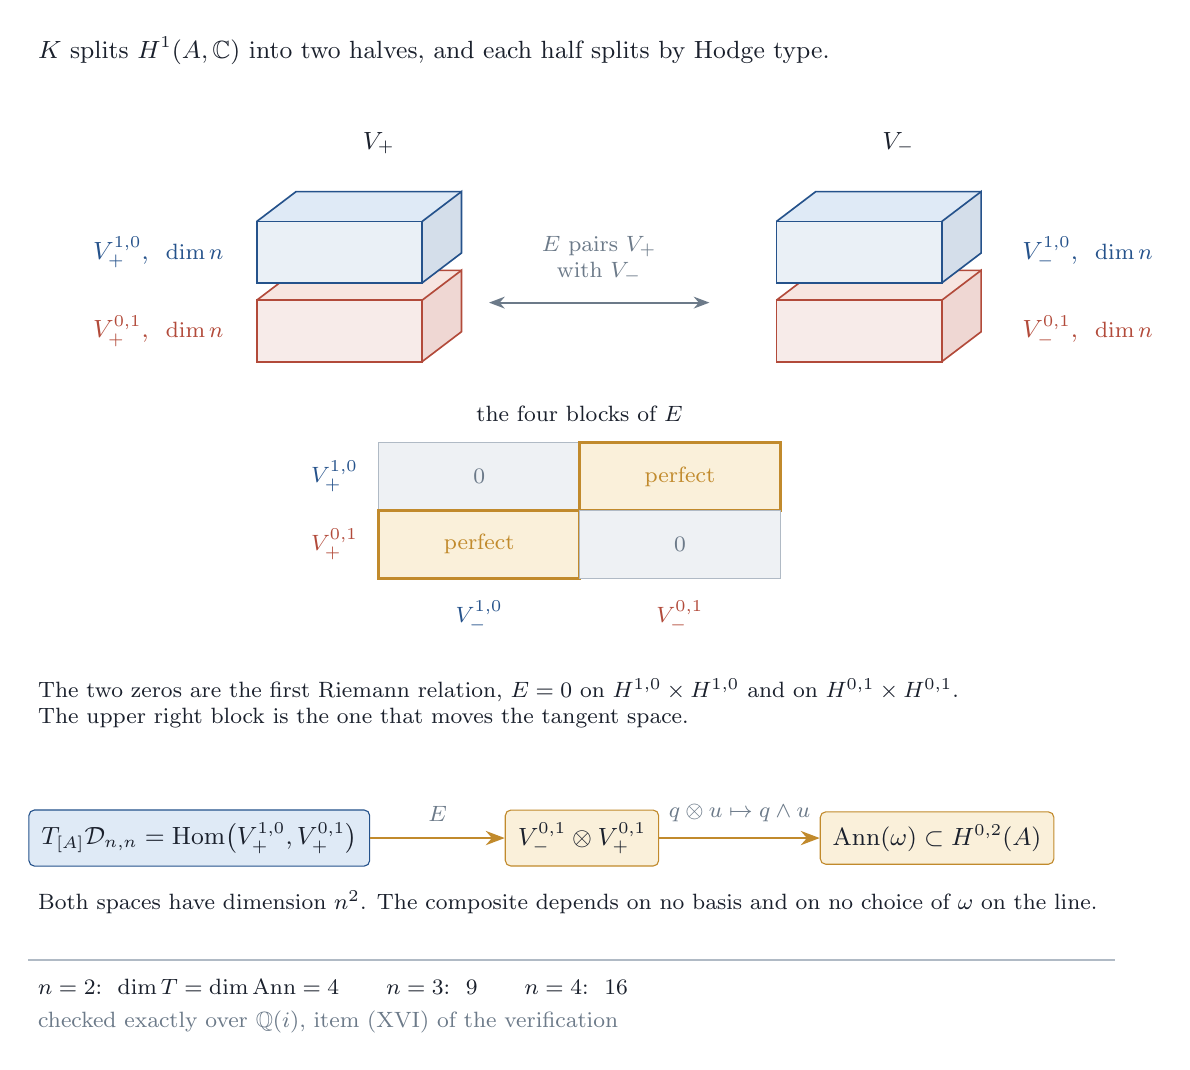
\begin{tikzpicture}[font=\small,text=PInk]

%% =====================================================================
%% Top: the two eigenspaces, each split by Hodge type.
%% =====================================================================
\node[anchor=west,font=\small,text=PInk] at (-2.9,3.95)
  {$K$ splits $H^{1}(A,\CC)$ into two halves, and each half splits by Hodge
   type.};

\slab{0}{0}{0}{2.1}{1.0}{0.78}{ahol}
\slab{0}{0}{1.00}{2.1}{1.0}{0.78}{hol}
\begin{scope}[obl]
  \coordinate (Lhi) at (0,0,1.39);
  \coordinate (Llo) at (0,0,0.39);
  \coordinate (Ltop) at (1.05,1.0,1.78);
\end{scope}
\node[anchor=east,align=right,text=PBlue] at ([xshift=-3mm]Lhi)
  {$V_{+}^{1,0}$, \ {\footnotesize $\dim n$}};
\node[anchor=east,align=right,text=PClay] at ([xshift=-3mm]Llo)
  {$V_{+}^{0,1}$, \ {\footnotesize $\dim n$}};
\node[anchor=south,font=\small,text=PInk] at ([yshift=3.5mm]Ltop) {$V_{+}$};

\slab{6.6}{0}{0}{2.1}{1.0}{0.78}{ahol}
\slab{6.6}{0}{1.00}{2.1}{1.0}{0.78}{hol}
\begin{scope}[obl]
  \coordinate (Rhi) at (8.7,0,1.39);
  \coordinate (Rlo) at (8.7,0,0.39);
  \coordinate (Rtop) at (7.65,1.0,1.78);
\end{scope}
\node[anchor=west,align=left,text=PBlue] at ([xshift=9mm]Rhi)
  {$V_{-}^{1,0}$, \ {\footnotesize $\dim n$}};
\node[anchor=west,align=left,text=PClay] at ([xshift=9mm]Rlo)
  {$V_{-}^{0,1}$, \ {\footnotesize $\dim n$}};
\node[anchor=south,font=\small,text=PInk] at ([yshift=3.5mm]Rtop) {$V_{-}$};

\node[anchor=center,align=center,font=\footnotesize,text=PSlate] at (4.35,1.30)
  {$E$ pairs $V_{+}$\\with $V_{-}$};
\draw[{Stealth[length=2mm]}-{Stealth[length=2mm]},PSlate,line width=0.8pt]
  (2.95,0.75) -- (5.75,0.75);

%% =====================================================================
%% The block matrix of E.  Nonzero on the antidiagonal only.
%% =====================================================================
\begin{scope}[shift={(1.55,-2.75)}]
  \def\cw{2.55}
  \def\ch{0.86}
  % cells: row 0 = V_+^{1,0}, row 1 = V_+^{0,1}; col 0 = V_-^{1,0}, col 1 = V_-^{0,1}
  \fill[WSlate] (0,\ch) rectangle (\cw,2*\ch);
  \draw[PRule,line width=0.5pt] (0,\ch) rectangle (\cw,2*\ch);
  \node[font=\footnotesize,text=PSlate] at (0.5*\cw,1.5*\ch) {$0$};

  \fill[WOchre] (\cw,\ch) rectangle (2*\cw,2*\ch);
  \draw[POchre,line width=1.1pt] (\cw,\ch) rectangle (2*\cw,2*\ch);
  \node[font=\footnotesize,text=POchre,align=center] at (1.5*\cw,1.5*\ch)
    {perfect};

  \fill[WOchre] (0,0) rectangle (\cw,\ch);
  \draw[POchre,line width=1.1pt] (0,0) rectangle (\cw,\ch);
  \node[font=\footnotesize,text=POchre,align=center] at (0.5*\cw,0.5*\ch)
    {perfect};

  \fill[WSlate] (\cw,0) rectangle (2*\cw,\ch);
  \draw[PRule,line width=0.5pt] (\cw,0) rectangle (2*\cw,\ch);
  \node[font=\footnotesize,text=PSlate] at (1.5*\cw,0.5*\ch) {$0$};

  \node[anchor=east,font=\footnotesize,text=PBlue] at (-0.14,1.5*\ch)
    {$V_{+}^{1,0}$};
  \node[anchor=east,font=\footnotesize,text=PClay] at (-0.14,0.5*\ch)
    {$V_{+}^{0,1}$};
  \node[anchor=north,font=\footnotesize,text=PBlue] at (0.5*\cw,-0.16)
    {$V_{-}^{1,0}$};
  \node[anchor=north,font=\footnotesize,text=PClay] at (1.5*\cw,-0.16)
    {$V_{-}^{0,1}$};

  \node[anchor=south,font=\footnotesize,text=PInk] at (\cw,2*\ch+0.14)
    {the four blocks of $E$};
\end{scope}

\node[anchor=north west,align=left,font=\footnotesize,text=PInk] at (-2.9,-3.90)
  {The two zeros are the first Riemann relation, $E=0$ on
   $H^{1,0}\times H^{1,0}$ and on $H^{0,1}\times H^{0,1}$.\\
   The upper right block is the one that moves the tangent space.};

%% =====================================================================
%% The chain of isomorphisms.
%% =====================================================================
\begin{scope}[shift={(0,-6.05)}]

\node[draw=PBlue,fill=WBlue,rounded corners=2pt,inner sep=4.5pt,
      anchor=west,align=center,text=PInk]
  (T) at (-2.9,0)
  {$T_{[A]}\mathcal{D}_{n,n}=\operatorname{Hom}\bigl(V_{+}^{1,0},V_{+}^{0,1}\bigr)$};

\node[draw=POchre,fill=WOchre,rounded corners=2pt,inner sep=4.5pt,
      anchor=west,align=center,text=PInk]
  (M) at (3.15,0)
  {$V_{-}^{0,1}\otimes V_{+}^{0,1}$};

\node[draw=POchre,fill=WOchre,rounded corners=2pt,inner sep=4.5pt,
      anchor=west,align=center,text=PInk]
  (A) at (7.15,0)
  {$\operatorname{Ann}(\omega)\subset H^{0,2}(A)$};

\draw[-{Stealth[length=2.4mm]},POchre,line width=1.0pt] (T) -- (M);
\draw[-{Stealth[length=2.4mm]},POchre,line width=1.0pt] (M) -- (A);
\node[anchor=south,font=\footnotesize,text=PSlate]
  at ($(T.east)!0.5!(M.west)+(0,0.08)$) {$E$};
\node[anchor=south,font=\footnotesize,text=PSlate]
  at ($(M.east)!0.5!(A.west)+(0,0.08)$) {$q\otimes u\mapsto q\wedge u$};

\node[anchor=north west,align=left,font=\footnotesize,text=PInk] at (-2.9,-0.55)
  {Both spaces have dimension $n^{2}$. The composite depends on no basis and
   on no choice of $\omega$ on the line.};

\end{scope}

%% =====================================================================
%% Bottom strip: the numbers, checked exactly.
%% =====================================================================
\begin{scope}[shift={(0,-8.20)}]
  \draw[PRule,line width=0.5pt] (-2.9,0.60) -- (10.9,0.60);
  \node[anchor=west,font=\footnotesize,text=PInk] at (-2.9,0.26)
    {$n=2$:\ \ $\dim T=\dim\operatorname{Ann}=4$\qquad
     $n=3$:\ \ $9$\qquad
     $n=4$:\ \ $16$};
  \node[anchor=west,font=\footnotesize,text=PSlate] at (-2.9,-0.18)
    {checked exactly over $\QQ(i)$, item (XVI) of the verification};
\end{scope}

\end{tikzpicture}
\end{document}
